\documentclass{article}
\title{Automaten en Berekenbaarheid:\\opgave 1}
\author{Prof. B. Demoen (\url{Bart.Demoen@cs.kuleuven.be})\\ W. Van Onsem (\url{Willem.VanOnsem@cs.kuleuven.be})}
\date{5 november 2013}
\usepackage{tikz,../assignment-nl}
\usetikzlibrary{automata,arrows,decorations.pathmorphing,backgrounds,positioning,fit}
\newcommand{\lang}[1]{\textsc{#1}}
\begin{document}
\maketitle
\paragraph{Richtlijnen}

Je schrijft enkel op de gekleurde bladen die je gekregen hebt: op je
werkplek liggen geen andere bladen dan die gekleurde bladen en de
bladen van de cursustekst. De bladen van je cursustekst waarop
oplossingen van oefeningen of aanwijzingen tot oplossingen van
oefeningen staan, steek je ook weg. Je jas, je boekentas, je gsm
... leg je vooraan in het auditorium, zoals gebruikelijk bij een
examen. Bij het afgeven zorg je dat je naam op je bladen staat, en dat
je alles aan elkaar niet. Er zijn 4 vragen.

\begin{question}[Pompend lemma voor reguliere talen]
Indien de voorgestelde taal niet regulier is: bewijs dit aan de hand van het pompend lemma voor reguliere talen. Indien
de voorgestelde taal dit wel is: geeft een reguliere expressie of een eindige toestandsautomaat die de taal
beschrijft/beslist.
\begin{enumerate}
 \item De verzameling strings uit $\Sigma=\accl{a,b}$ zodat voor elke string $s\in\Sigma^\star$, $s\in L$ indien voor
elke prefix\footnote{Een prefix van $s$ is een substring van $s$ die begint bij het eerste karakter van $s$ en op een
willekeurige plaats $k$ eindigt.} van $s$ het aantal $a$'s en $b$'s in de string nooit meer dan 2 verschilt.
 \item $L=\accl{a^mc^nb^m|m,n\in\NN\mbox{ met $m> n$}}$
 \item $L=\accl{a^mb^n|m,n\in\NN\mbox{ met $m<n$ en $m<981$}}$.
 \item $L=\accl{wv^\star w|v\in\Sigma,w\in\Sigma^\star}$ voor een willekeurige eindige $\Sigma$ die uit
minstens twee elementen bestaat.
\end{enumerate}
\end{question}
\begin{answer}[Pompend lemma voor reguliere talen]
We beschouwen de verschillende talen.
\begin{enumerate}
 \item Regulier. Vermits de eigenschap voor iedere prefix geldt, kunnen we een transitie-eigenschap uitbuiten: een string maakt nog kans om geaccepteerd te worden indien in het verleden het verschil nooit meer dan twee bedroeg. We beschouwen dus 5 accepterende toestanden die het verschil van -2 tot 2 opslaan. Telkens wanneer een $a$ of $b$ wordt uitgelezen, gaan we naar een toestand die \'e\'entje hoger of lager is. Wanneer we een $a$ lezen bij $-2$ of een $b$ bij $2$ komen we in een ongeldige toestand terecht. Deze zal de overige karakters inlezen zonder in een accepterende eindtoestand te eindigen.\\
 \begin{center}
 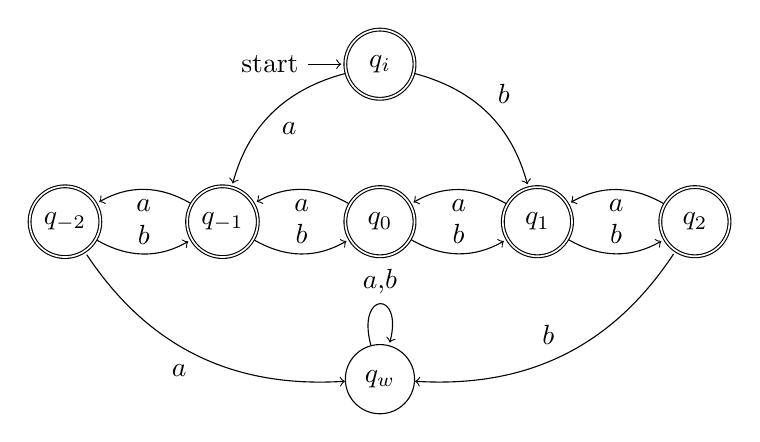
\begin{tikzpicture}[shorten >=1pt,node distance=2cm,on grid,auto]
 \node[state,initial,accepting]   (qi) {$q_i$};
 \node[state,accepting] (q0) [below=of qi] {$q_0$};
 \node[state,accepting] (q9) [left=of q0] {$q_{-1}$};
 \node[state,accepting] (q8) [left=of q9] {$q_{-2}$};
 \node[state,accepting] (q1) [right=of q0] {$q_1$};
 \node[state,accepting] (q2) [right=of q1] {$q_2$};
 \node[state]           (qw) [below=of q0] {$q_w$};
 \path[->] (qi) edge [bend right] node {$a$} (q9) edge [bend left] node {$b$} (q1);
 \foreach \i/\j in {8/9,9/0,0/1,1/2} {
   \path[->] (q\j) edge [bend right] node {$a$} (q\i);
   \path[->] (q\i) edge [bend right] node {$b$} (q\j);
 }
 \path[<-] (qw) edge [bend left] node {$a$} (q8) edge [bend right] node {$b$} (q2);
 \path[->] (qw) edge [loop above] node {$a$,$b$} ();
 \end{tikzpicture}
 \end{center}
 \item We beschouwen we de string $s=a^db^{d-1}c^d$. Voor deze string geldt dus $\abs{s}\geq d$ met $d$ de pomplengte. Voor elke indeling $s=xyz$ geldt dat $y$ uitsluitend uit $a$'s kan bestaan (vermits $\abs{xy}\leq d$ en $\abs{y}>0$). We kunnen dus besluiten dat $y=a^k$ met $k$ onbekend maar $0<k\leq d$. De taal is regulier wanneer voor elke $i$, $xy^iz\in L$, maar $xy^2z=a^{d+k}b^{d-1}c^d$, dit behoort duidelijk niet tot $L$, bijgevolg is de taal niet regulier.
 \item Regulier. We construeren eerst een reguliere expressie aan de hand van een parameter $i$:
 \begin{equation}
  a^ib^{i+1}b^\star
 \end{equation}
 Vervolgens is $L$ gelijk aan een eindige unie:
 \begin{equation}
  \displaystyle\bigcup_{i=0}^{980} a^ib^{i+1}b^\star
 \end{equation}
Concreet ziet de reguliere expressie er dus als volgt uit:
\begin{equation}
 bb^\star\ |\ abbb^\star\ |\ aabbbb^\star\ |\ aaabbbbb^\star\ |\ \cdots\ |\ \underbrace{aaaaa\cdots a}_{980\mbox{\small{ keer}}}\underbrace{bbbbbb\cdots b}_{981\mbox{\small{ keer}}}b^\star
\end{equation}
 \item Niet-regulier. Stel dat $a$ en $b$ twee elementen uit $\Sigma$ zijn\footnote{Hoe de symbolen eruit zien maakt niet uit, evenmin dat er nog andere symbolen betrokken zijn.}. In dat geval beschouwen we de string $s=a^dba^d$. Voor deze string geldt dus $\abs{s}\geq d$ met $d$ de pomplengte. Voor elke indeling $s=xyz$ geldt dat $y$ uitsluitend uit $a$'s kan bestaan (vermits $\abs{xy}\leq d$ en $\abs{y}>0$). We kunnen dus besluiten dat $y=a^k$ met $k$ onbekend maar $0<k\leq d$. De taal is regulier wanneer voor elke $i$, $xy^iz\in L$, maar $xy^2z=a^{d+k}bc^d$, dit behoort duidelijk niet tot $L$, bijgevolg is de taal niet regulier.
\end{enumerate}
\end{answer}
\begin{question}[Algebra van talen]
Niet alle talen behoren tot \emph{RegLan}, denk bijvoorbeeld aan $\lang{AGelijkB}=\accl{a^nb^n|n\in\NN}$. Stel dat $L_1$
en $L_2$ verschillende niet-reguliere talen zijn; en $L_3$ en $L_4$ verschillende oneindige reguliere talen niet gelijk
aan $\Sigma^*$ met $\Sigma$ het alfabet van de talen in kwestie. Zijn volgende talen dan regulier, niet-regulier of
hangt dit af van de talen in kwestie. Bewijs of geef tegenvoorbeelden.
\begin{enumerate}
 \item $L_1\cap L_3$.
 \item $L_1\cup L_3$.
 \item $L_1\cup L_2$.
 \item $\overline{L_1}\cup L_3$.
\end{enumerate}
\end{question}
\begin{answer}[Pompend lemma voor reguliere talen]
We beschouwen de verschillende talen.
\begin{enumerate}
 \item\label{itm:l1capl3} Hangt van de talen af:
 \begin{itemize}
  \item De doorsnede kan regulier zijn, bijvoorbeeld $L_1=\accl{a^mb^n|m\leq n}$ en $L_2=\accl{aab^ma^n|m\geq n}$, dan is $L_1\cap L_2=\accl{aabbb^\star}$ wat regulier is.
  \item De doorsnede kan niet-regulier zijn, bijvoorbeeld $L_1=\accl{a^mb^n|m\leq n}$ en $L_2=\accl{a^mb^n|m\geq n}$, dan is $L_1\cap L_2=\accl{a^mb^m|m\in\NN}$ wat niet-regulier is.
 \end{itemize}
 \item Hangt van de talen af:
 \begin{itemize}
  \item De unie kan regulier zijn, bijvoorbeeld: stel $L_1=\accl{a^mb^n|m\geq n}$ en $L_3=\accl{a^\star b^\star}$. De unie is $L_1\cup L_3=\accl{a^\star b^\star}$, deze taal is regulier.
  \item De unie kan niet-regulier zijn, bijvoorbeeld: stel $L_1=\accl{a^mb^n|m\geq n}$ en $L_3=\accl{aa^\star b}$. De unie is $L_1\cup L_3=\accl{a^mb^n|m\geq n}$, deze taal is niet-regulier.
 \end{itemize}
 \item Hangt van de talen af:
 \begin{itemize}
  \item De unie kan regulier zijn, bijvoorbeeld stel $L_1=\accl{a^mb^n|m\geq n}$ en $L_2=\accl{a^mb^n|m\leq n}$. De unie is $L_1\cup L_2=\accl{a^\star b^\star}$, deze taal is regulier.
  \item De unie kan niet-regulier zijn, bijvoorbeeld: stel $L_1=\accl{a^mb^n|m\geq n}$ en $L_2=\accl{a^mb^n|m> n}$. De unie is $L_1\cup L_2=\accl{a^mb^n|m\geq n}$, deze taal is niet-regulier.
 \end{itemize}
 \item Hangt van de talen af: vermits het complement van een reguliere taal, regulier is, weten we dat $\overline{L_1}$ ook niet-regulier is. Bijgevolg grijpen we terug naar de voorbeelden uit \ref{itm:l1capl3} om aan te tonen dat het van de talen afhangt.
\end{enumerate}
\end{answer}
\begin{question}[Pompend lemma voor contextvrije talen]
Indien de voorgestelde taal niet context-vrij is: bewijs dit aan de hand van het pompend lemma voor contextvrije talen.
Indien de voorgestelde taal dit wel is: geeft een reguliere expressie, een eindige toestandsautomaat, een contextvrije
grammatica of een push-down automaat die de taal beschrijft/beslist.
\begin{enumerate}
 \item $L=\accl{a^mb^nc^{n+m}|m,n\in\NN}$
 \item $L=\accl{a^mb^nc^md^n|m,n\in\NN}$
 \item $L_R=\accl{wv\hat{w}|w\in\Sigma^*\wedge v\in R}$ voor een willekeurige eindige $\Sigma$ die uit minstens twee
elementen bestaat en $R$ een reguliere taal over $\Sigma$.
\end{enumerate}
\end{question}
\begin{answer}[Pompend lemma voor contextvrije talen]
We beschouwen de verschillende talen.
\begin{enumerate}
 \item Context-vrij. Volgend push-down automaat beslist de taal:
 \begin{center}
 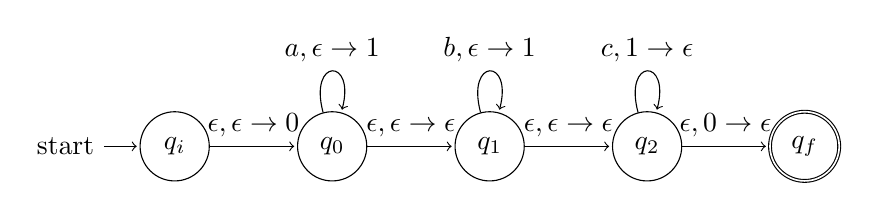
\begin{tikzpicture}[shorten >=1pt,node distance=2cm,on grid,auto]
 \node[state,initial]   (qi) {$q_i$};
 \node[state] (q0) [right=of qi] {$q_0$};
 \node[state] (q1) [right=of q0] {$q_1$};
 \node[state] (q2) [right=of q1] {$q_2$};
 \node[state,accepting] (qf) [right=of q2] {$q_f$};
 \path[->] (qi) edge node {$\epsilon,\epsilon\rightarrow 0$} (q0);
 \path[->] (q0) edge node {$\epsilon,\epsilon\rightarrow\epsilon$} (q1);
 \path[->] (q1) edge node {$\epsilon,\epsilon\rightarrow\epsilon$} (q2);
 \path[->] (q2) edge node {$\epsilon,0\rightarrow\epsilon$} (qf);
 \path[->] (q0) edge [loop above] node {$a,\epsilon\rightarrow 1$} ();
 \path[->] (q1) edge [loop above] node {$b,\epsilon\rightarrow 1$} ();
 \path[->] (q2) edge [loop above] node {$c,1\rightarrow \epsilon$} ();
 \end{tikzpicture}
 \end{center}
 \item Niet context-vrij. We beschouwen de string $s=a^pb^pc^pd^p$. Voor deze string geldt dus $\abs{s}\geq p$ met $p$ de pomplengte. Voor elke indeling $s=uvxyz$ geldt dat $v$ en $y$ uitsluitend uit \'e\'en soort karakters kunnen bestaan, indien niet zal men bij het pompen bijvoorbeeld na een sequentie $b$'s terug een sequentie $a$'s kunnen tegenkomen. Iets wat zeker niet tot de taal behoort. Bijgevolg kunnen we stellen dat $v=q^k$ en $y=r^l$ met $q,r\in\Sigma$. Omdat $\abs{vxy}\leq p$ weten we ook dat $v$ en $y$ minder dan $p$ plaatsen van elkaar gelegen moeten zijn. Dit betekent dus dat ofwel $q=r$ en beide delen dus eenzelfde sequentie van karakters bepalen. In dat geval kan de string niet gepompt worden: wanneer we immers $i$ verhogen ontstaat er een onbalans: stel dat we $q=r=a$ nemen dan zullen we met $i=2$, de string $a^{p+k+l}b^pc^pd^p$ genereren, wat duidelijk niet tot $L$ behoort. In een ander geval zijn de karakters verschillend: $q\neq r$. Stel $q=a$ en $r=b$, dan genereren we bij $i=2$ de string $a^{p+k}b^{p+l}c^pd^p$ dit behoort opnieuw niet tot $L$, dit laatste geldt ook voor andere segmenten zoals bijvoorbeeld $q=b$ en $r=c$.
 \item Context-vrij. $R$ is een reguliere taal, dus kan $R$ geschreven worden als een reguliere expressie $E$. We kunnen deze reguliere expressie inductief omzetten naar een contextvrije grammatica met startsymbool $R_E$ als volgt:
 \begin{itemize}
  \item Indien $E=\epsilon$, dan $R_E\rightarrow\epsilon$;
  \item Indien $E=a$ met $a\in\Sigma$, dan $R_E\rightarrow a$;
  \item Indien $E=E_1|E_2$ met $E_1$ en $E_2$ reguliere expressies, dan $R_E\rightarrow R_{E_1}$ en $R_E\rightarrow R_{E_2}$;
  \item Indien $E=E_1E_2$ met $E_1$ en $E_2$ reguliere expressies, dan $R_E\rightarrow R_{E_1}R_{E_2}$;
  \item Indien $E=\brak{E_1}^\star$ met $E_1$ een reguliere expressie, dan $R_E\rightarrow R_{E_1}R_E$ en $R_E\rightarrow \epsilon$;
  \item Indien $E=\phi$, dan defini\"eren we geen overgangsregel voor $R_E$.
 \end{itemize}
We bekomen dus een symbool $R_E$ die de taal van $R$ beschrijft. Vervolgens bouwen we volgende contextvrije grammatica:
\begin{itemize}
 \item Voor elke $a\in\Sigma$ defini\"eren we de regel: $S\rightarrow aSa$.
 \item We voorzien ook een regel $S\rightarrow R_E$.
\end{itemize}
De finale grammatica heeft als startsymbool $S$.
\end{enumerate}
\end{answer}
\begin{question}[Myhill-Nerode relaties]
Gegeven de volgende twee partities:
\begin{eqnarray}
P_1=\accl{\accl{a,b},\accl{c},\accl{d},\accl{e,f,g},\accl{h} }\\
P_2=\accl{\accl{a,e},\accl{b,c},\accl{d,h},\accl{f,g} }
\end{eqnarray}
Bepaal het supremum van de twee partities volgens de theorie in de cursus (sectie 13.3).
\end{question}
\begin{answer}[Myhill-Nerode relaties]
Het supremum is gedefinieerd als de \emph{fijnste relatie die grover is dan de originele relaties}. De resulterende relatie is dan:
\begin{equation}
P=\accl{\accl{a,b,c,e,f,g},\accl{d,h} }
\end{equation}
\end{answer}
\end{document}